\section{Construção de um exemplo}

Introdução à construção do exemplo.

\subsection{O estudo original}

O estudo original buscava avaliar o impacto de intervenções de psicologia positiva conduzidas via internet sobre a percepção de felicidade e
sintomas depressivos \cite{Woodworth2017}, uma tentativa de replicar os resultados obtidos em um trabalho anterior conduzido por Seligman e
colaboradores \cite{Seligman2005}.

\subsubsection{Participantes}

Os participantes foram recrutados por meio de anúncios em veículos de comunicação australianos: páginas web, jornais e uma estação de rádio
local. Um total de 295 participantes completou a fase inicial de pré-teste. O grupo era composto majoritariamente por mulheres ($85,06\%$),
com idades entre 18 e 83 anos ($M=43,76; SD=12,43$); a maior parte dos participantes possuia nível de educação superior ($74,88\%$) e classificou
a própria renda como média ou acima da média ($76\%$) \cite{Woodworth2017, Collins2023}.

\subsubsection{Intervenções}

Os participantes foram distribuídos aleatoriamente em quatro grupos, três grupos experimentais e um grupo de controle; cada um dos três grupos
experimentais recebeu uma intervenção distinta. O primeiro grupo experimental recebeu a intervenção de \emph{visita da gratidão}: os participantes
foram instruídos escrever e entregar uma carta de agradecimento para alguém que lhes tivesse sido gentil no passado. O segundo grupo experimental
recebeu a intervenção de \emph{três coisas boas}: os participantes deveriam anotar três coisas boas que haviam acontecido durante seu dia, justificando
suas escolhas de eventos. O último grupo experimental recebeu a intervenção de \emph{pontos fortes}: os participantes receberam uma intevenção
psicoeducativa sobre forças de caráter e foram aconselhados a buscar maneiras criativas para utilizar suas próprias forças de caráter no cotidiano.
Todas as intervenções tiveram duração de uma semana \cite{Woodworth2017}.

\subsubsection{Controle}

O grupo de controle foi exposto à atividade placebo de \emph{memórias de infância}: os participantes receberam a instrução de reservar um momento ao
final do dia para escrever sobre suas memórias de infância durante uma semana \cite{Woodworth2017}.

\subsubsection{Desfechos}

O estudo avaliou percepção de felicidade por meio do AHI (Authentic Happiness Inventory), um instrumento de autorrelato composto por 24 items. Os itens
são pontuados em uma escala de que vai de 1 a 5 e a pontuação total é calculada pela soma das pontuações obtidas para cada item. Resultados maiores representam
maiores níveis de felicidade \cite{Park2010}.

Sintomas depressivos foram mensurados com a escala CES-D (Center for epidemiologic studies depression scale), um instrumento de autorrelato composto por 20
itens que avaliam a frequência de sintomas em uma escala Likert de 4 pontos. A CES-D é divida em quatro subescalas: afeto deprimido, afeto positivo, queixas
somáticas e problemas interpessoais. A pontuação em uma subescala é calculada pela soma das pontuações obtidas para cada item associado à subescala. A pontuação
total é calculada pela soma das pontuações obtidas para cada subescala. Resultados maiores representam maior severidade dos sintomas depressivos \cite{Radloff1977}.

\subsection{Árvores de decisão}

Árvores de decisão representam uma classe de modelos de aprendizagem de máquina que pode ser usada para tarefas de classificação e regressão, ou seja, são
capazes de fazer predições para valores de variáveis categóricas e numéricas. Elas utilizam uma série de regras de decisão para predizer o desfecho de interesse;
essas regras consistem em verificações feitas sobre os valores de variáveis presentes no conjunto de dados de treinamento \cite{Theobald2021, Bi2019}.

\begin{figure}[h!]
    \centering
    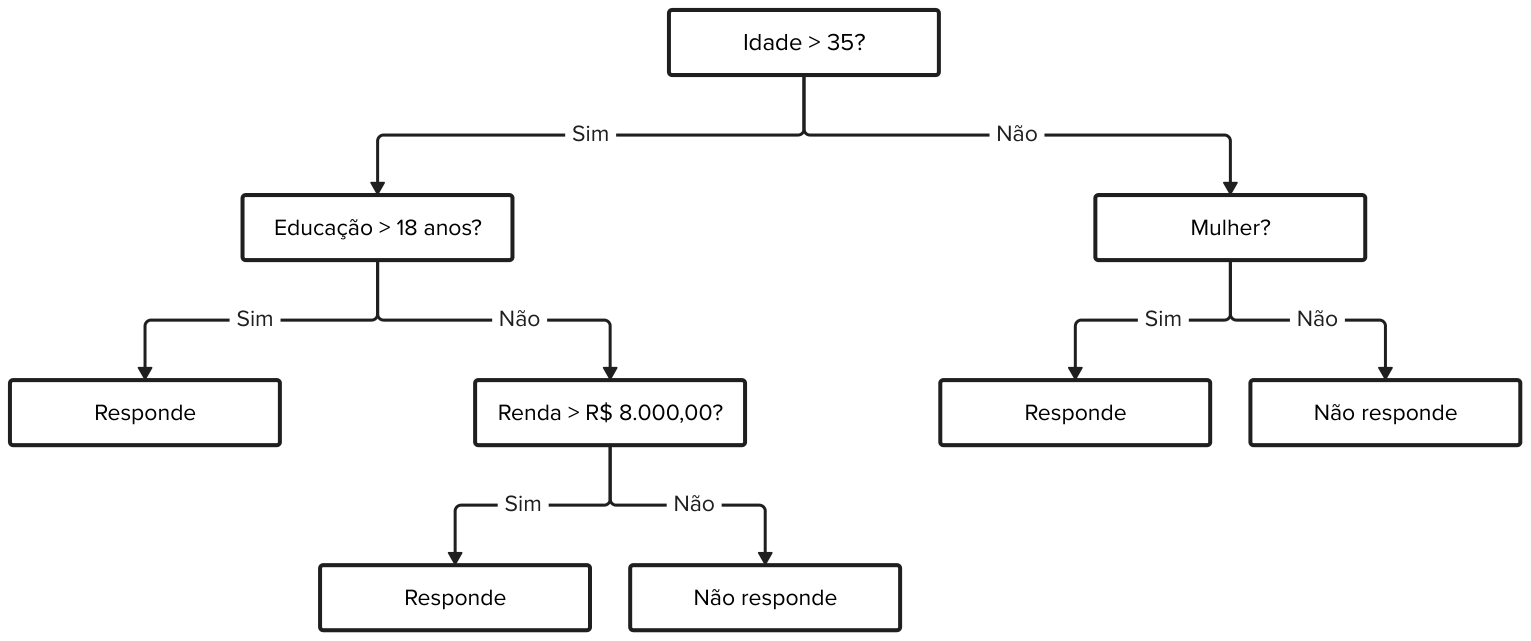
\includegraphics[width=\textwidth]{./03-exemplo/imagens/arvore-exemplo.png}
    \caption{Uma árvore de decisão hipotética para predição de resposta a determinada intervenção.}
    \label{fig:arvore-exemplo}
\end{figure}

\subsection{Plano de análise de dados}

A.

\subsection{Resultados e discussão}

A.
